\chapter{El aprendizaje de métricas de distancia} \label{chapter:dml_theory}

En este capítulo se describe el problema central de aprendizaje que se desarrolla en este trabajo. Para ello, se recordarán los conceptos de distancia y pseudodistancia, haciendo especial hincapié en aquellas distancias sobre espacios de Hilbert de dimensión finita. Estas distancias permitirán describir el problema del aprendizaje de métricas de distancia. Finalmente, se describen las aplicaciones de este paradigma de aprendizaje, destacando entre ellas el aprendizaje por semejanza, donde las distancias juegan un papel fundamental.

\section{Distancias. Distancia de Mahalanobis.}

\subsection{Definición y ejemplos}

El concepto de distancia es fundamental en el paradigma de aprendizaje que vamos a desarrollar. En primer lugar recordamos la definición de distancia y espacio métrico.

\begin{definition}[Distancia]
    Sea $X$ un  conjuntono vacío. Una \emph{distancia} o \emph{métrica} definida sobre $X$ es una aplicación $d:X\times X \to \mathbb{R}$, verificando las siguientes propiedades:
    
    \begin{enumerate}
        \item $d(x,y)=0  \iff x = y $, para todos $x,y \in X$ (Coincidencia) \label{item:dist:coincid}
        \item $d(x,y)=d(y,x)$, para todos  $x,y \in X$ (Simetría)  \label{item:dist:sim}
        \item $d(x,z)\le d(x,y)+d(y,z)$, para todos $x,y,z \in X$ (Desigualdad triangular) \label{item:dist:triang}
    \end{enumerate}
    
    Al par ordenado $(X,d)$ se le denomina espacio métrico.
\end{definition}

\begin{remark}
    Como consecuencia de la definición se tienen las siguientes propiedades adicionales.
    \begin{enumerate}
        \setcounter{enumi}{3}
        \item $d(x,y) \ge 0 \ \forall x,y \in X$ (No negatividad) \label{item:dist:no_neg}
        \item $|d(x,y)-d(y,z)| \le d(x,z) \ \forall x,y,z \in X$ (Desigualdad triangular por defecto) \label{item:dist:triang_def}
        \item $d(x_1,x_n) \le \sum_{i=1}^{n-1}d(x_i,x_{i+1}) \ \forall x_1,\dots,x_n \in X$ (Desigualdad triangular generalizada) \label{item:dist:triang_gen}
    \end{enumerate}
\end{remark}

\begin{proof}
    $ $ \newline
    \begin{enumerate}
        \setcounter{enumi}{3}
        \item $ 0 \us{\ref{item:dist:coincid}}{=} \frac{1}{2}d(x,x) \us{\ref{item:dist:triang}}{\le}\frac{1}{2}[d(x,y)+d(y,x)]\us{\ref{item:dist:sim}}{=}d(x,y) \ \forall x,y \in X$
        
        \item Usando $\ref{item:dist:sim}$ y $\ref{item:dist:triang}$ se tiene:
        \[d(x,y) \le d(x,z) + d(z,y) = d(x,z)+d(y,z) \implies d(x,y)-d(y,z)\le d(x,z)\]
        \[d(y,z) \le d(y,x) + d(x,z) = d(x,y)+d(x,z) \implies d(y,z)-d(x,y)\le d(x,z) \]
        Por tanto podemos tomar valores absolutos en la diferencia obteniendo la desigualdad buscada.
        
        \item Es consecuencia de la desigualdad triangular aplicando inducción.
    \end{enumerate}
\end{proof}

Veamos algunos de los ejemplos más conocidos de espacios métricos.

\begin{example}[Subespacios métricos]
Sea $(X,d)$ un espacio métrico y $A\subset X$. La aplicación $d_{|A}:A\times A \to \mathbb{R}^+_0$ es una distancia, y $(A,d_{|A})$ es un subespacio métrico de $(X,d)$.
\end{example}

\begin{example}[Distancia trivial]
    Sea $X$ cualquier conjunto no vacío. Sobre $X$ definimos la aplicación $d:X\times X \to \mathbb{R}^+_0$ por
    \[d(x,y):= \begin{cases}
    0 & \text{, si } x = y \\
    1 & \text{, si } x \ne y
    \end{cases}.\]
    $(X,d)$ es un espacio métrico, y $d$ es una distancia trivial que nos indica solo si dos elementos de $X$ son iguales o distintos.
\end{example}

\begin{example}[Distancia de Hamming]
    Sean $(X_i,d_i), i=1,\dots, n$ espacios métricos con distancias triviales. Consideramos $X = X_1 \times \dots \times X_n$, $x = (x_1,\dots,x_n), y = (y_1,\dots,y_n) \in X$ y la aplicación $d:X\times X \to \mathbb{R}^+_0$ dada por
    \[d(x,y) = \sum_{i=1}^n d(x_i,y_i).\]
    La aplicación $d$ es una distancia que nos muestra el número de elementos que difieren entre dos vectores $x,y$ de $X$, y se conoce como distancia de Hamming. Es muy utilizada en algunos ámbitos de la teoría de la información, y es la distancia mas popular sobre espacios cuyas componentes no son ordenables.
\end{example}

\begin{example}[Distancias asociadas a normas] \label{ex:dist:norm}
    Si $(X,\|.\|)$ es un espacio normado real, se define la distancia asociada a la norma por $d(x,y)=\|x-y\|$ para todos $x,y\in X$. Las distancias asociadas a normas verifican propiedades adicionales, de combrobación inmediata:
    \begin{enumerate}
        \setcounter{enumi}{6}
        \item $d(ax,ay) = |a|d(x,y)$, para $a \in \R$, $x,y \in X$ (homogeneidad) \label{item:dist:homogen}
        \item $d(x,y) = d(x+z,y+z)$ para $x,y,z \in X$ (invarianza por traslaciones) \label{item:dist:inv_tras}
    \end{enumerate}
    Profundizaremos sobre estas distancias en las siguientes secciones.
\end{example}

\subsection{Pseudodistancias}

El concepto de distancia se puede suavizar, relajando la condición de coincidencia, obteniendo así lo que se conoce como una pseudodistancia, una aplicación que mantiene muchas de las propiedades de una distancia, y en muchos campos, como el que vamos a tratar, puede aplicarse con la misma utilidad que las distancias. De hecho, veremos que en algunos casos una pseudodistancia puede tener propiedades más beneficiosas que una distancia propia. Veamos su definición y algunos ejemplos y propiedades.

\begin{definition}[Pseudodistancia]
    Sea $X$ un conjunto no vacío. Una \emph{pseudodistancia} definida sobre $X$ es una aplicación $d:X\times X \to \mathbb{R}^{+}_{0}$, verificando las siguientes propiedades:
    
    \begin{enumerate}
        \item $d(x,x)=0$, para todo $x \in X$ \label{item:pdist:coincid}
        \item $d(x,y)=d(y,x)$, para todos $x,y \in X$ (Simetría) \label{item:pdist:sim} 
        \item $d(x,z)=d(x,y)+d(y,z)$, para todos $x,y,z \in X$ (Desigualdad triangular) \label{item:pdist:triang}
    \end{enumerate}
    
\end{definition}

Podemos ver que el único cambio de la definición consiste en eliminar una de las implicaciones en la propiedad \ref{item:dist:coincid} (ahora puede haber elementos distintos con distancia nula entre ellos). Este cambio no afecta a la demostración de las propiedades $\ref{item:dist:no_neg}$, $\ref{item:dist:triang_def}$ y $\ref{item:dist:triang_gen}$ de la distancia, luego estas siguen siendo válidas en las pseudodistancias. Veamos algunos ejemplos de pseudodistancias.

\begin{example}[Ejemplos básicos]
    \begin{enumerate}
        \item Toda distancia sobre $X$ es una pseudodistancia sobre $X$.
        \item La aplicación nula $d:X\times X \to \mathbb{R}^+_0$ dada por $d(x,y) = 0 \ \forall x,y \in X$ es una pseudodistancia.
    \end{enumerate}
\end{example}

\begin{example}[Espacios de funciones integrables]

Sea $\Omega \subset \mathbb{R}$ y consideramos, para $1 < p < \infty$, los espacios de funciones integrables 
\[L^p(\Omega)=\left\{f\colon\Omega \to \mathbb{R} \colon f \text{ es medible y } \int_{\Omega} |f(t)|^p dt < \infty \right\}.\]

Dadas $f,g \in L^p(\Omega)$ definimos la pseudodistancia entre ellas como \[d(f,g)=\left(\int_{\Omega}|f(t)-g(t)|^p dt\right)^{1/p}.\]

Es claro que se verifican las propiedades $\ref{item:pdist:coincid}$ y $\ref{item:pdist:sim}$ de pseudodistancia, y la $\ref{item:pdist:triang}$ es una aplicación directa de la desigualdad integral de Minkowski. Sin embargo, no es una distancia puesto que si $d(f,g)=0$ solo tenemos asegurada la igualdad casi por doquier.

\end{example}

\begin{example}[Pseudodistancias asociadas a seminormas]
    Si $X$ es un espacio vectorial real y $\|.\|$ es una seminorma, se define la distancia asociada a la seminorma por $d(x,y)=\|x-y\| \ \forall x,y\in X$. Estas pseudodistancias verifican también las propiedades $\ref{item:dist:homogen}$ y $\ref{item:dist:inv_tras}$ que verifican las distancias asociadas a normas. Profundizaremos sobre ellas en la siguiente sección.
\end{example}

Para concluir esta sección, vamos a mostrar que a partir de una pseudodistancia podemos definir una relación de equivalencia mediante la cual, tras identificar los elementos en las mismas clases, podemos obtener un espacio métrico.

\begin{prop}
    Sea $X$ un conjunto no vacío y $d:X\times X \to \mathbb{R}^+_0$ una pseudodistancia sobre $X$. Definimos la relación $x \sim y \iff d(x,y)=0$. $\sim$ es una relación de equivalencia.
\end{prop}

\begin{proof}~
\begin{itemize}
    \item \emph{Reflexiva.} Consecuencia de la propiedad $\ref{item:pdist:coincid}$ de pseudodistancia.
    \item \emph{Simétrica.} Consecuencia de la propiedad $\ref{item:pdist:sim}$ de pseudodistancia.
    \item \emph{Transitiva.} Consecuencia de la propiedad $\ref{item:pdist:triang}$ de pseudodistancia.
\end{itemize}

\end{proof}

\begin{thm} \label{thm:quotient_dist}

En las condiciones anteriores, el cociente $X/_\sim$ es un espacio métrico con la distancia $\hat{d}:X/_\sim \times X/_\sim \to \mathbb{R}^+_0$ dada por $\hat{d}([x],[y])=d(x,y) \ \forall[x],[y] \in X/_\sim$

\end{thm}

\begin{proof}

En primer lugar veamos que la aplicación $\hat{d}$ está bien definida. Para ello veamos que la distancia no depende del representante escogido. Supongamos $[x]=[x']$ y $[y]=[y']$ (lo que implica que $d(x,x')=0=d(y,y')$. Queremos ver que $d(x,y)=d(x',y')$. Aplicamos varias veces la desigualdad triangular.

\[d(x,y)\le \ub{d(x,x')}_{=0}+d(x',y) \le d(x',y')+\ub{d(y',y)}_{=0}\]
\[\le \ub{d(x',x)}_{=0}+d(x,y') \le d(x,y) + \ub{d(y,y')}_{=0} \]

Por tanto, $d(x,y) \le d(x',y') \le d(x,y)$, obteniendo la igualdad. Que $\hat{d}$ es una distancia es inmediato por la definición de la relación de equivalencia y las propiedades de $d$.

\end{proof}

De los ejemplos anteriores podemos obtener los primeros espacios métricos a partir de cocientes:

\begin{itemize}
    \item Si $(X,d)$ es un espacio métrico, la relación de equivalencia es la igualdad y el espacio cociente es esencialmente idéntico a $(X,d)$.
    \item Para cualquier conjunto $X$ no vacío, la pseudodistancia nula origina el espacio cociente de un solo punto, donde la aplicación nula sí es una distancia.
    \item Los espacios cociente de los $L^p$ bajo la relación dada por la pseudodistancia anterior (en este caso es la igualdad c.p.d.) son los conocidos espacios de Banach de funciones integrables $\mathcal{L}^p$
\end{itemize}

\subsection{Distancias de Mahalanobis}

Dentro de los espacios normados de dimensión finita nos encontramos con un conjunto de pseudodistancias muy útiles en el campo de la computación. Estas vienen dadas por matrices semidefinidas positivas, e independientemente de si se tratan de distancias propias o únicamente de pseudodistancias, se les conoce como distancias de Mahalanobis.

\begin{definition}
    Sea $d \in \N$ y $M \in \mathcal{M}_d(\R)^+_0$. La \emph{distancia de Mahalanobis} asociada a la matriz $M$ es la aplicación $d_M \colon \R^d \times \R^d \to \R^+_0$, dada por
    \[d_M(x,y) = \sqrt{(x-y)^TM(x-y)}. \]
\end{definition}

Es claro que $d_M$ es una pseudodistancia, pues esta pseudodistancia procede de la seminorma $\|x\|_M = \sqrt{x^TMx}$, que a su vez procede del (pseudo-)producto escalar $\langle x, y \rangle_M = x^TMy$. Por tanto, cuando $M$ es definida positiva, $d_M$ da a $\R^d$ una estructura de espacio de Hilbert. Observemos que el espacio euclídeo usual está incluido en estos espacios, y se presenta cuando $M = I$.

En ocasiones se emplea el término \emph{distancia de Mahalanobis} refiriéndose a la distancia al cuadrado, $d_M^2$. En el ámbito de la computación es mucho más eficiente trabajar con $d_M^2$ que con $d_M$, pues se evita así el cálculo de las raíces cuadradas. Aunque $d_M^2$ no sea realmente una distancia, mantiene las propiedades más útiles de $d_M$ desde el punto de vista de la computación, como por ejemplo, la mayor o menor cercanía entre distintas parejas de puntos. Por eso está bastante extendido el uso de \emph{distancia de Mahalanobis} tanto para $d_M$ como para $d_M^2$.

Como hemos comentado, las distancias de Mahalanobis inducen (salvo aquellas que no verifican la propiedad de coincidencia) una estructura de espacio de Hilbert en $\R^d$. El recíproco también es cierto, puesto que toda forma bilineal simétrica en $\R^d$ viene determinada por una matriz simétrica. Si la forma es además semidefinida positiva (induciendo una pseudodistancia) también lo será la matriz, y si la forma es definida positiva (siendo por tanto un producto escalar), la matriz asociada será también definida positiva. Por tanto, todos los productos escalares (incluyendo aquellos semidefinidos) vienen determinados por marices semidefinidas positivas.

Finalmente, al igual que las pseudodistancias inducían espacios métricos en el cociente, lo mismo ocurre con las distancias asociadas a matrices semidefinidas positivas singulares. En este caso dicho cociente implica una reducción de la dimensión del espacio, como vamos a ver a continuación. Esto es de nuevo una ventaja computacional, pues permitirá trabajar con datos de menor tamaño.

\begin{prop} \label{prop:mahalanobis_lowrank}
    Sea $d_M$ una distancia de Mahalanobis en $\R^d$. Entonces,
    \begin{enumerate}
        \item $V = \{x \in \R^d \colon d_M(x,0) = \|x\|_M = 0 \}$ es un subespacio vectorial de $\R^d$.
        \item Si $\dim(V) = m$, $\R^d / V$ es un espacio vectorial de dimensión $d' = d - m$, que como conjunto cociente es igual a $\R^d/\sim$ ($\sim$ es la relación de equivalencia del teorema \ref{thm:quotient_dist})
        \item $d_M$ induce en $\R^d / V$ una distancia de Mahalanobis $d_{M'}$, donde $M' \in \mathcal{M}_{d'}(\R)$ es definida positiva.
    \end{enumerate}
\end{prop}

\begin{proof}~
    \begin{enumerate}
        \item Sean $u, v \in V, \lambda, \mu \in \R$. Entonces,
        \[0 \le \|\lambda u + \mu v \|_M \le \|\lambda u \|_M+\|\mu v\|_M = |\lambda|\|u\|_M+|\mu|\|v\|_M = 0, \]
        luego $\|\lambda u + \mu v\|_M = 0$ y $\lambda u + \mu v \in V$.

        \item Recordemos que la relación de equivalencia definida por un subespacio vectorial viene dada por $x \sim_V y \iff x - y \in V$, los elementos en el cociente son de la forma $V \in [x] = x+ V := \{x+v \colon v \in V\}$, y la suma y producto por escalares vienen dados por $[x] + [y] = [x+y], a[x] = [ax]$, para $x,y \in \R^d$, $a \in \R$. La comprobación de que estas operaciones no dependen del representante es inmediata. 

        La aplicación $p\colon \R^d \to \R^d/V$ dada por $p(x) = [x]$ es lineal, gracias a la definición de las operaciones en el cociente, y sobreyectiva. Además,
        \[\ker(p) = \{x \in \R^d \colon x + V = V \} = \{x \in \R^d \colon x \in V  \} = V. \]
        Por tanto,
        \[ \dim(\R^d/V) = \dim(\im(p)) = \dim(\R^d) - \dim(\ker(p)) = \dim(\R^d) - \dim(V) = d - m.\]
        Finalmente, observamos que $\sim_{V} = \sim$ debido a la invarianza por traslaciones de las pseudodistancias asociadas a normas. Si $x,y \in \R^d$,
        \[ x \sim_{V} y \iff x-y \in V \iff d_M(x-y,0) = 0 \iff d_M(x,y) = 0  \iff x \sim y.\]

        \item Llamamos $U = \R^d/V$. Definimos la aplicación $\langle \cdot, \cdot \rangle \colon U \times U \to \R$ por $\langle x +V, y+V \rangle = x^TMy$. Veamos que $\langle \cdot, \cdot \rangle$ es un producto escalar.
        \begin{itemize}
            \item Está bien definida. Si $x+V = x'+V \in U$ e $y+V=y'+V \in U$, entonces $x-x' \in V, y-y' \in V$, luego $\|x-x'\|_M = \|y-y'\|_M = 0$. Observemos que
            \begin{align*}
            \langle x+V, y+V \rangle - \langle x' + V, y' + V \rangle &= x^TMy - (x')^TMy + (x')^TMy - (x')^TM(y') \\
                                &= (x - x')^TMy + (x')^TM(y - y').  
            \end{align*}
            La deigualdad de Cauchy-Schwarz \ref{thm:cauchy_schwarz} obliga a que los últimos sumandos sean 0, puesto que $\|x-x'\|_M = \|y-y'\|_M = 0$. En consecuencia, $\langle x+V, y+V \rangle = \langle x' + V, y' + V \rangle$.

            \item Es lineal. Si $\lambda, \mu \in \R$ y $x+V,y+V,z+V \in U$,
            \begin{align*}
             \langle \lambda(x+V) + \mu(y+V), z + V \rangle &= \langle (\lambda x + \mu y + V), z + V \rangle = (\lambda x + \mu y)^TMz \\
                                            & = \lambda(x^TMz)+\mu(y^TMz) = \lambda\langle x+V,z+V \rangle + \mu\langle y+V,z+V \rangle.
            \end{align*}
            \item Es simétrica. Si $x+V,y+V \in U$,
            \[ \langle x + V, y+V \rangle = x^TMy = (x^TMy)^T = y^TM^Tx = y^TMx = \langle y + V, x+V\rangle. \]

            \item Es definida positiva. Si $x + V \in U$, $\langle x + V, x + V \rangle = x^TMx \ge 0$, y
            \[ \langle x + V, x + V \rangle = 0 \iff x^TMx = 0 \iff \|x\|_M = 0 \iff x \in V \iff x+V = 0+V, \]
            luego $\langle x + V, x + V \rangle = 0$ si y solo si $x+V$ es el neutro en el espacio cociente, concluyendo que $\langle \cdot, \cdot \rangle$ es un producto escalar.
        \end{itemize}

        Por tanto, por ser un producto escalar, fijando una base ortonormal en $U$ y suponiendo los vectores en $U$ con coordenadas en dicha base, existe una matriz definida positiva $M' \in \mathcal{M}_{d'}(\R)$ tal que $\langle x+V, y+V \rangle = (x+V)^TM'(y+V)$. Para concluir, basta ver que la distancia inducida por $M'$ es la distancia inducida por $d$ sobre el cociente. En efecto, si consideramos la distancia $\hat{d}\colon U \times U \to \R^+_0$ dada por el teorema \ref{thm:quotient_dist}, se tiene
        \[\hat{d}(x+V,y+V)^2 = d(x,y) = (x-y)^TM(x-y) = \langle (x-y)+V, (x-y)+V \rangle = d_{M'}^2(x+V,y+V).\]

    \end{enumerate}
\end{proof}


\section{Descripción del problema}
    Uno de los componentes más importantes en muchos procesos cognitivos del ser humano consiste en la capacidad para detectar parecidos o semejanzas entre distintos objetos. Esta capacidad se ha llevado al campo del aprendizaje automático mediante el diseño de algoritmos que aprenden de un conjunto de datos de acuerdo con las similaridades entre dichos datos.

    Para medir la similaridad entre los datos, es necesario introducir una distancia, la cual nos permite establecer una medida de cercanía mediante la cual se puede determinar cuándo un par de puntos es más similar que otro par de puntos. Sin embargo, como hemos visto en la sección anterior, existe una infinidad de distancias con las que podemos trabajar, y es posible que no todas ellas se adapten correctamente a nuestros datos, y no sean adecuadas para detectar las semejanzas entre estos. Por eso, la elección de una distancia adecuada es un elemento crucial en este tipo de algoritmos. La búsqueda de una distancia apropiada es la tarea que se lleva a cabo en el aprendizaje de métricas de distancia.

    El \emph{aprendizaje de métricas de distancia} (\emph{DML}, \emph{Distance Metric Learning}) es una disciplina del aprendizaje automático cuya finalidad es aprender distancias (incluyendo pseudodistancias, aunque no se indique explícitamente) a partir de un conjunto de datos. En su versión más general, se dispone de un conjunto de datos $\mathcal{X} = \{x_1,\dots,x_N\}$, sobre el que se han recogido determinadas medidas de similitud entre distintos pares o tripletas de datos. Dichas similitudes vienen determinadas por los conjuntos
    \begin{align*}
        S &= \{(x_i,x_j) \in \mathcal{X}\times\mathcal{X} \colon x_i \text{ y } x_j \text{ son similares.} \} \\
        D &= \{(x_i,x_j) \in \mathcal{X}\times\mathcal{X} \colon x_i \text{ y } x_j \text{ no son similares.} \} \\
        R &= \{(x_i,x_j,x_l) \in \mathcal{X}\times\mathcal{X}\times\mathcal{X} \colon x_i \text{ es más similar a } x_j \text{ que a } x_l. \}.
    \end{align*}
    Con estos datos y conjuntos de similitud, el problema a resolver consiste en, fijada una familia de distancias $\mathcal{D}$, encontrar aquellas que mejor se adapten a los criterios especificados por los conjuntos de similitud. Para ello, se fija una determinada función de pérdida $\ell$, y las distancias buscadas serán aquellas que resuelvan el problema de optimización
    \[ \min_{d \in \mathcal{D}} \ell(d,S,D,R) .\]
    La selección de distintas funciones de pérdida es lo que conduce a las distintas técnicas de aprendizaje de métricas de distancia. Cada una de dichas funciones permitirá elaborar una determinada estrategia de optimización. Estos aspectos, para el caso del aprendizaje supervisado, se estudiarán en el siguiente capítulo.

    A continuación vamos a concretar la descripción del problema. En primer lugar, si nos centramos en el aprendizaje supervisado, especialmente en el orientado a clasificación, además del conjunto $\mathcal{X}$ de datos, dispondremos de una lista de etiquetas $y_1,\dots,y_N$ asociadas a cada dato. En este caso, la formulación general del problema se adapta fácilmente a la nueva situación, sin más que considerar los conjuntos $S$ y $D$ como
    \begin{align*}
        S &= \{(x_i,x_j) \in \mathcal{X}\times\mathcal{X} \colon y_i = y_j\} \\
        D &= \{(x_i,x_j) \in \mathcal{X}\times\mathcal{X} \colon y_i \ne y_j\} 
    \end{align*}
    Adicionalmente, se puede disponer del conjunto $R$ definiendo tripletas $(x_i,x_j,x_l)$, donde en general $y_i = y_j \ne y_l$, verificándose además determinadas condiciones sobre la distancia entre $x_i$ y $x_j$, frente a la distancia entre $x_i$ y $x_l$. Este es el caso, por ejemplo, de los impostores en el algoritmo LMNN (véase la sección \ref{section:lmnn}). En cualquier caso, las etiquetas disponen de toda la información necesaria en el ámbito del aprendizaje de métricas supervisado. En adelante nos centraremos en problemas de este tipo.

    Por otro lado, centrándonos en la naturaleza del conjunto de datos, prácticamente la totalidad de la teoría del aprendizaje de métrica de distancias se desarrolla para datos numéricos, debido en parte a la riqueza de las distancias de las que disponen y a su facilidad para ser parametrizadas computacionalmente, y en parte a que los datos de naturaleza nominal pueden ser convertidos a variables numéricas binarias u ordinales con un preprocesamiento adecuado. Por ello, nos centraremos de ahora en adelante en problemas de aprendizaje supervisado con datos numéricos.

    Supongamos entonces que $\mathcal{X} \subset \R^d$. Como vimos en la sección anterior, para espacios vectoriales de dimensión finita podemos tomar la familia de distancias de Mahalanobis, $\mathcal{D} = \{d_M \colon M \in \mathcal{M}_d(\R)^+_0\}$. Con esta familia tenemos a nuestra disposición todas las distancias asociadas a productos escalares en $\R^d$ (y en menores dimensiones para el caso de las pseudodistancias), y viene determinada por el conjunto de las matrices semidefinidas positivas, y por ello, podemos utilizar estas matrices para parametrizar las distancias. De esta forma, el problema general adaptado al aprendizaje supervisado con distancias de Mahalanobis podemos reescribirlo como
    \begin{equation} \label{eq:metric_learning_eq}
        \min_{M \in \mathcal{M}_{d}(\mathbb{R})^+_0} \ell(d_M,(x_1,y_1),\dots,(x_N,y_N)) .
    \end{equation}

    Sin embargo, esta no es la única forma de parametrizar este tipo de problemas. Sabemos, por el teorema \ref{thm:psd_decomposition} que si $M \in \mathcal{M}_d(\R)^+_0$, existe una matriz $L \in \mathcal{M}_d(\R)$ tal que $M = L^TL$ y dicha matriz es única salvo una isometría. Entonces se tiene que
    \[d_M^2(x,y) = (x-y)^TM(x-y) =(x-y)^TL^TL(x-y) = (L(x-y))^T(L(x-y)) = \|L(x-y)\|_2^2. \]

    Por tanto, podemos parametrizar las distancias también mediante cualquier matriz, aunque en este caso la interpretación es distinta. Cuando aprendemos distancias mediante matrices semidefinidas positivas estamos aprendiendo una nueva métrica sobre $\R^d$. Cuando los aprendemos mediante las matrices $L$ anteriores, estamos aprendiendo una aplicación lineal que transforma los datos en el espacio, y la distancia asociada es la distancia euclídea usual de los datos proyectados en el nuevo espacio. Ambos enfoques son equivalentes gracias al teorema \ref{thm:psd_decomposition}.

    En cuanto a la dimensionalidad, es importante destacar que cuando la métrica aprendida $M$ no tiene rango máximo, realmente estamos aprendiendo una distancia sobre un espacio de dimensión inferior (por la proposición \ref{prop:mahalanobis_lowrank}), lo que nos permite reducir la dimensionalidad de nuestro conjunto de datos. Lo mismo ocurre cuando aprendemos aplicaciones lineales $L$ que no tienen rango máximo. Podemos extender este caso y optar por aprender matrices $L \in M_{d'\times d}(\R)$, con $d' < d$. De esta forma, aseguramos que los datos se proyectan directamente a un espacio de dimensión no superior a $d'$.

    Ambos enfoques, tanto el de aprender la métrica $M$ como el de aprender la transformación $L$, son de gran utilidad para parametrizar los problemas del aprendizaje de métricas de distancia, cada uno con sus ventajas e inconvenientes. Por ejemplo, las parametrizaciones a través de $M$ suelen conducir a problemas de optimización convexos. En cambio, la convexidad en los problemas parametrizados por $L$ no es tan fácil de conseguir. Por otra parte, las parametrizaciones a través de $L$ permiten aprender directamente proyecciones a espacios de menor dimensión, mientras que las restricciones de dimensión para los problemas parametrizados por $M$ no son fáciles de satisfacer. Veamos estas diferencias con ejemplos sencillos.

    \begin{example}
        Muchas de las funciones que querremos optimizar dependerán de la distancia al cuadrado definida por la métrica $M$ o por la transformación $L$, es decir, o bien tendrán términos de la forma $\|v\|_M^2 = v^TMv$ o bien de la forma $\|v\|_L^2 = \|Lv\|_2^2$. Tanto la aplicación $M \mapsto \|v\|_M^2$ como la aplicación $L \mapsto \|v\|_L^2$ son convexas (la primera es, de hecho afín). Sin embargo, si queremos restar términos de esta forma, perdemos la convexidad en $L$, pues la aplicación $L \mapsto -\|v\|_L^2$ no es convexa. En cambio, la aplicación $M \mapsto -\|v\|_M^2$ sigue siendo afín y, por tanto, convexa.
    \end{example}

    \begin{example}
        Las restricciones de rango no son convexas, y por tanto no disponemos de una proyección convexa sobre dicha restricción para hacer cumplir dichas restricciones durante el proceso de aprendizaje, salvo que aprendamos directamente la proyección (parametrizada por $L$)  al espacio con la dimensión deseada. Por ejemplo, si consideramos el conjunto $C = \{ M \in \mathcal{M}_2(\R)^+_0 \colon r(A) \le 1 \}$, se tiene que $A = \begin{pmatrix} 2 & 0 \\ 0 & 0 \end{pmatrix} \in C$ y $B = \begin{pmatrix} 0 & 0 \\ 0 & 2 \end{pmatrix} \in C$. Sin embargo, $(1-\lambda)A+\lambda B = I \notin C$, para $\lambda=1/2$. 
    \end{example}

\section{Aplicaciones} \label{section:aplicaciones}

En esta sección se describen algunas de las principales aplicaciones del aprendizaje de métricas de distancia, ilustradas con algunos ejemplos.


\begin{itemize}
    \item \textbf{Mejorar la actuación de clasificadores basados en distancias.} Esta es una de las principales finalidades del aprendizaje de métricas supervisado. Mediante dicho aprendizaje, se encuentra una distancia que se adapte bien a los datos y al clasificador, mejorando el rendimiento de este último. En la figura \ref{fig:mejorar_knn} se muestra un ejemplo.

    \begin{figure}[h]
    \centering
    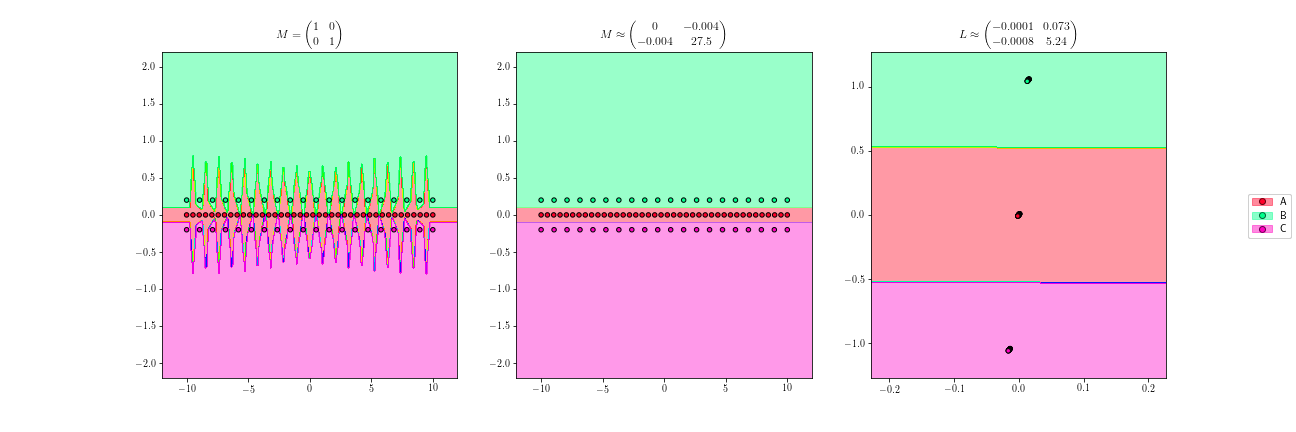
\includegraphics[width=21cm,center]{./images/ex_learning_nca.png}
    \caption{Supongamos que tenemos un conjunto de datos en el plano, los cuales pueden pertenecer a tres clases distintas, cuyas regiones vienen definidas por rectas paralelas. Supongamos que para clasificar un nuevo dato lo hacemos asignándole la clase del punto que se encuentre más cerca, para la distancia euclídea usual. Entonces, para los datos observados obtendríamos unas regiones de clasificación como las de la figura de la izquierda, pues los datos de las clases B y C están mucho más separados entre sí que la separación entre las regiones. Sin embargo, si aprendemos una distancia adecuada y volvemos a intentar clasificar asignando la clase del punto más cercano para esta nueva distancia, obtenemos unas regiones de clasificación como las de la figura central, mucho más efectivas. Por último, aprender una métrica es equivalente a aprender una transformación de los datos y medir en el espacio transformado con la distancia euclídea usual. Esto se muestra en la figura derecha. También podemos observar que los datos se están proyectando, salvo errores de precisión, sobre una recta, luego también estamos reduciendo la dimensionalidad del conjunto de datos.} \label{fig:mejorar_knn}
    \end{figure}
    
    \item \textbf{Reducción de la dimensionalidad.} Como ya hemos comentado, aprender una métrica de rango no máximo implica una reducción de dimensionalidad sobre los datos con los que trabajamos. Dicha reducción de dimensionalidad proporciona numerosas ventajas, como la reducción del coste computacional, tanto en espacio como en tiempo, de los algoritmos que se utilizarán posteriormente, o la eliminación del posible ruido introducido al tomar los datos. También, como veremos en la próxima sección, algunos algoritmos basados en distancias están expuestos a un problema denominado \emph{maldición de la dimensionalidad}. Reduciendo la dimensión de los datos, dicho problema también se hace menos grave. Por último, si se estima necesario, las proyecciones a dimensión 1,2 y 3 nos permitirían obtener representaciones visuales de nuestros datos, como se muestra en la figura \ref{fig:reduc_dim}

    \begin{figure}[h]
    \centering
    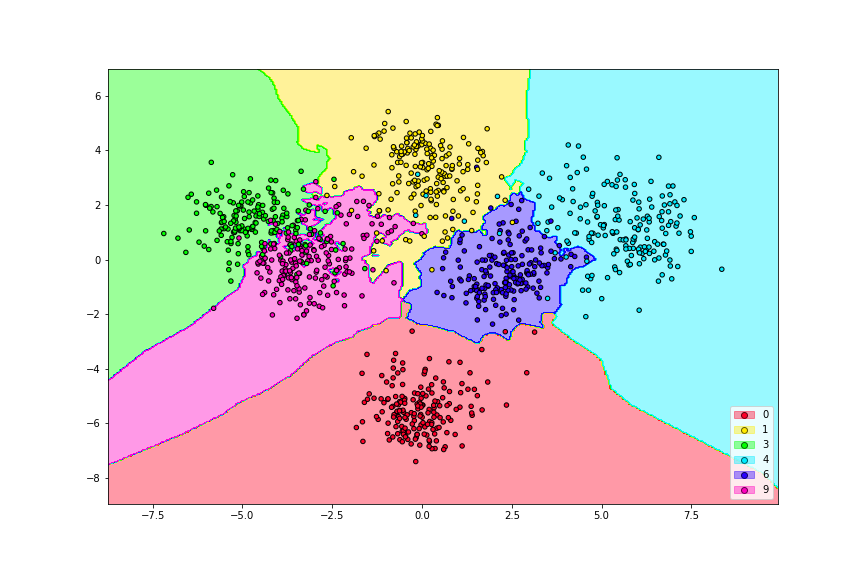
\includegraphics[width=0.75\textwidth]{./images/ex_red_dim.png}
    \caption{El dataset 'Dígitos' está formado por 1797 ejemplos. Cada uno de ellos consiste en un vector de 64 atributos, representando valores de intensidad sobre una imagen 8x8. Los ejemplos pertenecen a 10 clases distintas, cada una de ellas representando los números del 0 al 9. Aprendiendo una transformación adecuada somos capaces de proyectar la mayoría de clases sobre el plano, de forma que se perciban regiones claramente diferenciadas asociadas a cada una de las clases.} \label{fig:reduc_dim}
    \end{figure}


    \item \textbf{Cambio de ejes y reorganización de los datos.} Muy relacionada con la reducción de dimensionalidad, esta aplicación se debe a aquellos algoritmos que aprenden transformaciones que permiten mover (o seleccionar según la dimensión) los ejes de coordenadas, de forma que en el nuevo sistema de coordenadas los vectores concentren determinadas medidas de información en sus primeras componentes. Un ejemplo se muestra en la figura \ref{fig:mover_ejes}.

    \begin{figure}[h]
    \centering
    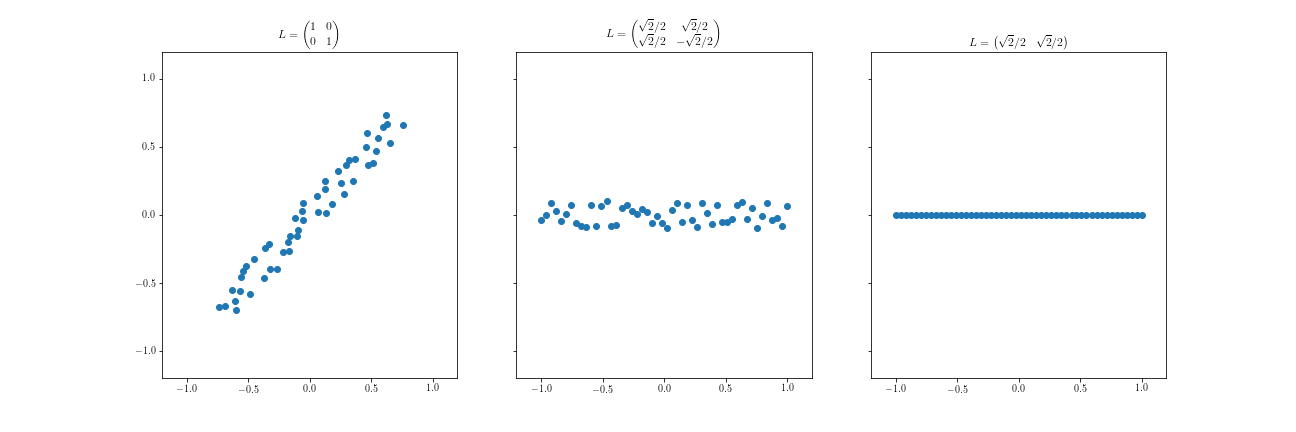
\includegraphics[width=20cm,center]{./images/ex_mover_ejes.png}
    \caption{El conjunto de datos de la figura izquierda parece que concentra la mayoría de su información en la recta diagonal que une las esquinas inferior izquierda y la superior derecha. Aprendiendo la transformación adecuada, podemos conseguir que dicha dirección caiga sobre el eje horizontal, como se muestra en la figura central. De esta forma, la primera coordenada de los vectores en esta nueva base concentra gran parte de la variabilidad del vector. Además, parece razonable pensar que los valores que introduce la coordenada vertical pueden deberse a ruido, por lo que podemos incluso quedarnos únicamente con la primera componente, como se muestra en la figura derecha.} \label{fig:mover_ejes}
    \end{figure}

    \item \textbf{Mejorar la actuación de los algoritmos de clustering.} Muchos de los algoritmos de clustering utilizan una distancia para medir la cercanía entre los datos, y así establecer los agrupamientos de forma que los datos presentes en un mismo grupo son cercanos para dicha distancia. En ocasiones, aunque desconozcamos los agrupamientos ideales de los datos ni el número de clusters a establecer, sí podemos saber que determinados pares de puntos deben estar en un mismo cluster y que otros determinados pares deben estar en clusters distintos. Esto ocurre en numerosos problemas, como por ejemplo, en el agrupamiento de documentos web. Dichos documentos poseen gran cantidad de información adicional, como es el caso de los links entre documentos, la cual nos puede incluirse como restricciones de similitud.

    \item \textbf{Aprendizaje semisupervisado.} El aprendizaje semisupervisado es un modelo de aprendizaje en el que se dispone de un conjunto de datos etiquetados y otro conjunto (en general mucho más grande) de datos sin etiquetar. Con ambos conjuntos de datos se busca aprender un modelo que permita etiquetar nuevos datos. El aprendizaje semisupervisado surge debido a que en muchas ocasiones la recopilación de datos sin etiquetar es relativamente sencilla, pero la asignación de etiquetas puede requerir que un supervisor las tenga que asignar manualmente, lo que puede ser inviable. En cambio, cuando se utilizan muchos datos no etiquetados junto con una pequeña cantidad de datos etiquetados es posible mejorar considerablemente los resultados del aprendizaje, como se ejemplifica en la figura \ref{fig:ssl}. Muchas de estas técnicas consisten en construir un grafo con aristas ponderadas a partir de los datos, donde el valor de las aristas depende de las distancias entre los datos. A partir de dicho grafo se trata de inferir las etiquetas de todo el conjunto de datos, mediante distintos algoritmos de propagación \cite{ssl1,ssl2}. En la construcción del grafo la elección de una distancia adecuada es importante, entrando así en juego el aprendizaje de métricas de distancia.

    \begin{figure}[h]
    \centering
    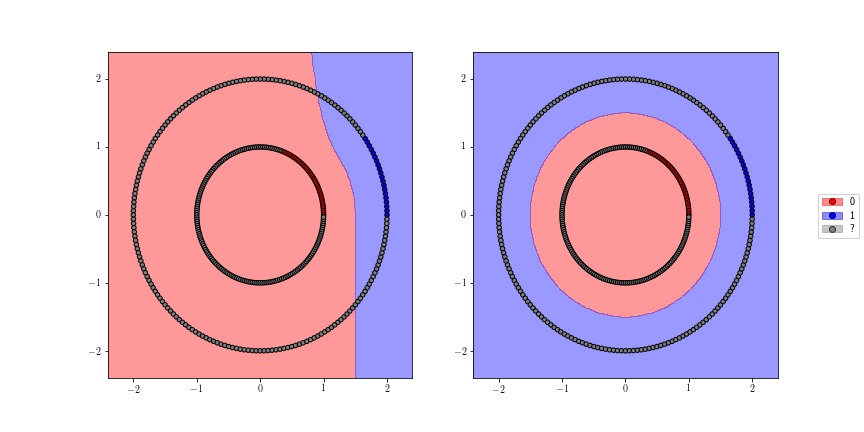
\includegraphics[width=\textwidth]{./images/ssl.png}
    \caption{Aprendizaje con la información supervisada (izquierda) frente al aprendizaje considerando toda la información no supervisada (derecha).} \label{fig:ssl}
    \end{figure}

\end{itemize}

Los algoritmos de aprendizaje supervisado analizados en este trabajo se centran en las tres primeras aplicaciones de la enumeración anterior.

\section{El aprendizaje por semejanza}

\subsection{Introducción}

El aprendizaje por semejanza es una disciplina del aprendizaje automático cuya finalidad es aprender a partir de la similitud con los datos en el conjunto de entrenamiento. De nuevo la similitud vendrá determinada por una función de distancia, por lo que el aprendizaje de una métrica apropiada previa a este proceso de aprendizaje aumentará la eficacia de este tipo de técnicas. De hecho, el aprendizaje por semejanza es una de las principales aplicaciones del aprendizaje de métricas de distancia, como se mostró en el primer ejemplo de la sección \ref{section:aplicaciones}.

En el aprendizaje supervisado, el enfoque que sigue este paradigma es el que se muestra a continuación. Supongamos que queremos aprender un clasificador para un conjunto de datos que se distribuyen de acuerdo a una distribución $\mathcal{D}$ de probabilidad. Disponemos para ello de una muestra $(x_1,y_1),\dots,(x_N,y_N)$ de datos etiquetados mediante una función de etiquetado desconocida $f\colon \mathcal{X} \to \mathcal{Y}$. Suponemos también que en el espacio $\mathcal{X}$ disponemos de una distancia $d$. Para un nuevo dato $x \sim \mathcal{D}$, le asignamos su clase a través de una función $h \colon \mathcal{X} \to \mathcal{Y}$ dada por $h(x) = \phi(d,x,(x_1,y_1),\dots,(x_N,y_N))$, una función que depende únicamente de los datos y de la distancia entre ellos.

Notemos que en este tipo de aprendizaje no buscamos un clasificador $h$ en una familia de hipótesis $\mathcal{H}$, de forma que se minimice una determinada función, sino que partimos de una función $h$ prefijada. Esto hace que el proceso de aprendizaje propiamente dicho consista únicamente en almacenar los datos en memoria, mientras que el esfuerzo computacional se realiza durante el proceso de predicción, en el que se evalúa la función de distancia. Este tipo de clasificadores, en los que el proceso de aprendizaje o generalización se retrasa hasta el momento en el que se desea predecir un nuevo dato, se denominan \emph{clasificadores perezosos}.

Por último, es interesante observar cómo el aprendizaje de métricas de distancia complementa a este tipo de clasificadores perezosos. Como ya hemos dicho, las técnicas de aprendizaje por semejanza no tienen un proceso de aprendizaje propiamente dicho y parten de una función hipótesis predefinida. En cambio, el aprendizaje de métricas de distancia sí parte de un conjunto de hipótesis, en concreto, el conjunto de distancias de Mahalanobis, como se mostraba en la expresión \ref{eq:metric_learning_eq}. Podemos combinar ambas técnicas obteniendo así un clasificador por semejanza que durante el aprendizaje encuentra una función hipótesis, dependiente de una distancia, que minimiza una función de pérdida definida para el conjunto de distancias de Mahalanobis.

El clasificador por semejanza más popular es el de vecinos cercanos, que analizaremos en la siguiente sección.

\subsection{El clasificador de vecinos cercanos.}

El clasificador de vecinos cercanos es un clasificador por semejanza muy conocido y que, como su propio nombre indica, clasifica los nuevos datos de acuerdo con la clase de sus vecinos más cercanos. Supongamos que tenemos la muestra de entrenamiento $(x_1,y_1),\dots,(x_N,y_N)$ y un dato a predecir, $x \in \mathcal{X}$. Definimos, para dicho $x$, una permutación $(\pi_1(x),\dots,\pi_N(x))$ del conjunto $\{1,\dots,N\}$ de forma que los datos de entrenamiento quedan ordenados por dicha permutación según su distancia a $x$, es decir, se tiene que
\[ d(x,x_{\pi_i}(x)) \le d(x,x_{\pi_{i+1}}(x)) \quad i=1,\dots,N-1. \]

Entonces, el clasificador de los $k$ vecinos cercanos o k-NN asigna a $x$ el valor más repetido en la lista $(y_{\pi_1(x)},\dots,y_{\pi_k(x)})$, es decir, la clase mayoritaria de sus $k$ vecinos más cercanos. Cuando $k=1$, la función hipótesis $h$ viene dada por $h(x) = y_{\pi_1}(x)$. En este caso, las regiones que determinan cada posible vecino más cercano vienen determinadas por politopos convexos (la generalización de polígonos y poliedros) y se denominan celdas de Voronoi. En el caso bidimensional, las regiones se pueden visualizar mediante diagramas de Voronoi (figura \ref{fig:voronoi}).

\begin{figure}[h]
    \centering
    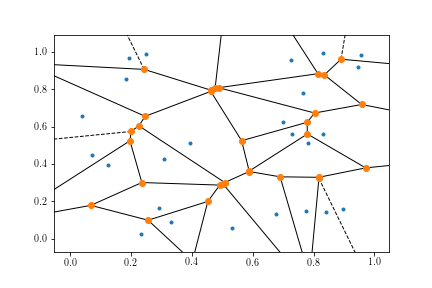
\includegraphics[width=0.5\textwidth]{./images/voronoi.png}
    \caption{Diagrama de Voronoi.} \label{fig:voronoi}
\end{figure}

Es interesante destacar que, por cómo se asignan las clases para los nuevos datos, el k-NN permite trabajar en problemas de clasificación multiclase sin ningún tipo de limitación. Esto, normalmente, no es así para muchos clasificadores, los cuales están diseñados únicamente para resolver problemas de clasificación binarios. Para extender estos clasificadores a problemas multiclase, la estrategia más común es dividir el problema en subproblemas binarios, resolver estos problemas, y asignar la clase final como aquella mayoritaria obtenida en los subproblemas. Los métodos usuales de división en problemas binarios consisten en enfrentar una clase frente a todas las demás (\emph{One versus All}), o enfrentar todos los pares de clases entre sí (\emph{One versus One}) \cite{ovoova}. En general, la mayoría de técnicas que aprenden por semejanza permiten también trabajar directamente con problemas multiclase.

La elección del número de vecinos $k$ puede influir bastante en la región delimitada por el clasificador. Dicha región es no paramétrica, al no hacerse ninguna asunción sobre la forma de la función hipótesis $h$. Los valores pequeños de $k$  se ajustan más a los datos de entrenamiento, generando así una región más puntiaguda. En tales casos, el sesgo es bajo pero la variabilidad es alta. Los papeles se intercambian para valores grandes de $k$, donde la región generada presenta un aspecto más suave, como se muestra en la figura \ref{fig:knn_comp_k}.

\begin{figure}[h]
    \centering
    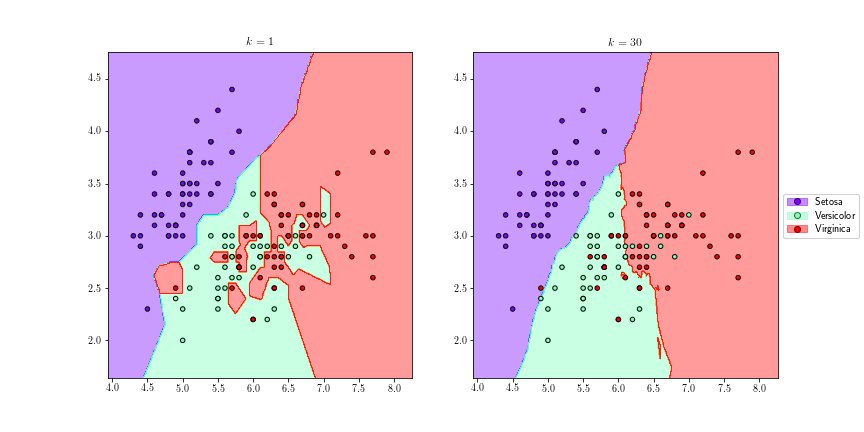
\includegraphics[width=\textwidth]{./images/compare_knn.png}
    \caption{Comparación del k-NN para distintos valores de $k$ (dataset 'Iris')} \label{fig:knn_comp_k}
\end{figure}

Como ya se anticipó en la sección, el k-NN sufre de la conocida como \emph{maldición de la dimensionalidad}. Nos restringimos al caso $k=1$. Supongamos que el dominio del problema es $\mathcal{X} = [0,1]^d$ (es decir, trabajamos con datos normalizados) y suponemos que el conjunto de clases es $\mathcal{Y} = \{0,1\}$. Suponemos que $\mathcal{D}$ es una distribución sobre $\mathcal{X}\times\mathcal{Y}$ para la cual la distribución de probabilidad condicionada, $\eta(x) = \mathbb{P}[y=1|x]$ es $c$-lipschitziana para la distancia $d$ con la que trabajamos. Entonces, es posible probar que la diferencia entre el error empírico y el \emph{error bayesiano óptimo}, asociado a la hipótesis $h^*(x) = \mathbbm{1}_{[\eta(x) > 1/2]}$ puede acotarse por $4c \sqrt{d} N^{-\frac{1}{d+1}}$ \cite{understandingml}, donde $N$ es el tamaño del conjunto de entrenamiento. Por tanto, si queremos asegurar que dicho error sea menor que $\varepsilon$, necesitamos escoger $N \ge (4c\sqrt{d}/\varepsilon)^{d+1}$. Es decir, según esta cota, el número de ejemplos crece exponencialmente con la dimensionaldad del conjunto. Además, es posible encontrar distribuciones para las cuales esta cota sea necesaria, además de suficiente. Esta circunstancia se puede generalizar para cualquier $k$, y es lo que se conoce como la maldición de la dimensionalidad para el k-NN. 

Por último, es importante comentar que se puede cambiar la regla de clasificación del k-NN. Por ejemplo para, en lugar de asignar la clase mayoritaria en los $k$ vecinos más cercanos, establecer una ponderación sobre cada vecino de forma inversamente proporcional a la distancia, teniendo así más peso las clases de los primeros vecinos más cercanos. También se puede extender esta regla a problemas de regresión, considerando por ejemplo la media, o una media ponderada, entre los $k$ vecinos más cercanos. En general, un clasificador o regresor de $k$ vecinos cercanos utiliza una función hipótesis que se puede expresar genéricamente como
\[ h(x) = \phi(x,d,(x_{\pi_1(x)},y_{\pi_1(x)}),\dots,(x_{\pi_N(x)},y_{\pi_N(x)})). \]

\subsection{Otros clasificadores por semejanza.}

Aunque el k-NN es el algoritmo por semejanza más popular para clasificación, no es el único. A continuación se muestran otros clasificadores relevantes.

\begin{itemize}
    \item \textbf{El clasificador de la media más cercana.} Denominado NCM (\emph{Nearest Class Mean}), este clasificador, durante el proceso de aprendizaje, calcula los vectores media de cada clase. Después, a la hora de predecir un nuevo dato, le asigna la clase del vector media más cercano. Es un clasificador muy eficiente y simple, aunque su simplicidad lo convierte en un clasificador bastante débil frente a conjuntos que no se agrupan en torno a su media. Existe la posibilidad de generalizarlo a múltiples centroides, como veremos en la sección \ref{section:ncmc}.

    \item \textbf{El clasificador de vecinos cercanos por radio}. Este clasificador es muy similar al k-NN, solo que en este caso, en vez de fijar un número de vecinos $k$, se fija un radio $R$. A la hora de clasificar un nuevo dato $x$, se buscan todos los datos del conjunto de entrenamiento que disten de $x$ menos que $R$. Todos los datos encontrados serán los vecinos cercanos de $x$, y a $x$ se le asignará la clase mayoritaria entre dichos vecinos. Notemos que en este caso, el número de vecinos varía con cada ejemplo, pudiendo incluso no haber vecinos. En este caso, la elección de un radio adecuado es muy importante, y puede presentar un comportamiento inadecuado en conjuntos de datos con grandes variaciones de densidad (podría haber zonas en las que apenas hay vecinos y zonas con un número elevado de vecinos).


\end{itemize}

\begin{comment}
\subsection{Fundamentos estadísticos del k-NN. La maldición de la dimensionalidad.}
\end{comment}
